%!TEX program = pdflatex
\documentclass[UTF8]{article}

\usepackage[UTF8]{ctex}
\usepackage{amsmath}
\usepackage{enumerate}
\usepackage{amssymb}
\usepackage{graphicx}
\usepackage{booktabs}
 
\title{Homework 3}
\author{陈旻 SA18225036}
\date{}
\begin{document}
\maketitle
\section{第6章 高级加密标准AES}
\paragraph{6.3}
What is the difference between Rijndael and AES?

Rijndael allows for block lengths of 128, 192, or 256 bits. AES allows only a block length of 128 bits.

\paragraph{6.14}
What is the difference between the AES decryption algorithm and the equivalent inverse cipher?

or the AES decryption algorithm, the sequence of transformations for decryption differs from that for encryption, although the form of the key schedules for encryption and decryption is the same. The equivalent version has the same sequence of transformations as the encryption algorithm (with transformations replaced by their inverses). To achieve this equivalence, a change in key schedule is needed.

\section{第7章 分组加密的工作模式}
\paragraph{7.1}
What is triple encryption?

With triple encryption, a plaintext block is encrypted by passing it through an encryption algorithm; the result is then passed through the same encryption algorithm again; the result of the second encryption is passed through the same encryption algorithm a third time. Typically, the second stage uses the decryption algorithm rather than the encryption algorithm.

\paragraph{7.2}
What is a meet-in-the-middle attack?

This is an attack used against a double encryption algorithm and requires a known (plaintext, ciphertext) pair. In essence, the plaintext is encrypted to produce an intermediate value in the double encryption, and the ciphertext is decrypted to produce an intermediation value in the double encryption. Table lookup techniques can be used in such a way to dramatically improve on a brute-force try of all pairs of keys.

\paragraph{7.3}
How many keys are used in triple encryption?

Triple encryption can be used with three distinct keys for the three stages; alternatively, the same key can be used for the first and third stage.
\paragraph{7.4}
List and briefly define the block cipher modes of operation.

\begin{enumerate}[(a)]
    \item ECB, 分组后分别加密。
    \item CBC, 加密时把上一个分组的密文和当前分组的明文异或后输入给AES算法,输出作为密文。
    \item CFB, 当s和block相同时:把上一个分组的密文输入给AES算法,用输出和当前分组的明文异或得到密文。当s小于block时:引入寄存器,把aes的出取s位和明文异或,得到s位的密文,并把这s位的密文存到寄存器中,并挤出最旧的s位。 寄存器的值作为aes的输入。
    \item OFB,当s和block相同时:把上一个分组的AES输出输入给AES算法,用输出个当前分组的明文异或得到密文。当s小于block时:也是用跟cfb类似的寄存器方式,区别是aes输出里的s位存到寄存器。
    \item CTR,把计数器的值输入给AES算法,用输出和当前分组的明文异或得到密文。
\end{enumerate}
\paragraph{7.5a}
Why do some block cipher modes of operation only use encryption while others use both encryption and decryption?

In some modes, the plaintext does not pass through the encryption function, but is XORed with the output of the encryption function. The math works out that for decryption in these cases, the encryption function must also be used.
\paragraph{7.5b}
为什么3DES的中间部分采用了解密而不是加密?

Encrypt-decrypt-encrypt (EDE) is the preferred method because if a single key is used for all 3 operations it is equivalent to regular 56-bit DES. That is, a 56-bit DES implementation can decrypt that message. This makes this version of 3DES backwards compatible with DES.

Encrypt-encrypt-encrypt (EEE) is also a valid method though. It is no more or less valid than EDE. However, EDE is usually preferred for the reasons mentioned above.
\paragraph{7.4}
With the ECB mode, if there is an error in a block of the transmitted ciphertext, only the corresponding plaintext block is affected. However, in the CBC mode, this error propagates. For example, an error in the transmitted C1(Figure 7.4) obviously corrupts P1 and P2.

\subparagraph{a}
Are any blocks beyond P2 affected?

No. For example, suppose C1 is corrupted. The output block P3 depends only on the input blocks C2 and C3.

\subparagraph{b}
Suppose that there is a bit error in the source version of P1. Through how many ciphertext blocks is this error propagated? What is the effect at the receiver?

An error in P1 affects C1. But since C1 is input to the calculation of C2, C2 is affected. This effect carries through indefinitely, so that all ciphertext blocks are affected.  However, at the receiving end, the decryption algorithm restores the correct plaintext for blocks except the one in error. You can show this by writing out the equations for the decryption. Therefore, the error only effects the corresponding decrypted plaintext block.
\paragraph{7.8}
If a bit error occurs in the transmission of a ciphertext character in 8-bit CFB mode, how far does the error propagate?

Nine plaintext characters are affected.  The plaintext character corresponding to the ciphertext character is obviously altered. In addition, the altered ciphertext character enters the shift register and is not removed until the next eight characters are processed.
\section{第9章 公钥密码学与RSA}
\paragraph{9.1}
What is a public key certificate?

A public-key certificate contains a public key and other information, is created by a certificate authority, and is given to the participant with the matching private key. A participant conveys its key information to another by transmitting its certificate. Other participants can verify that the certificate was created by the authority.
\paragraph{9.2}
What are the roles of the public and private key?

A user's private key is kept private and known only to the user. The user's public key is made available to others to use. The private key can be used to encrypt a signature that can be verified by anyone with the public key. Or the public key can be used to encrypt information that can only be decrypted by the possessor of the private key.
\paragraph{9.3}
What are three broad categories of applications of public-key cryptosystems?

Encryption/decryption: The sender encrypts a message with the recipient's public key. Digital signature: The sender "signs" a message with its private key. Signing is achieved by a cryptographic algorithm applied to the message or to a small block of data that is a function of the message. Key exchange: Two sides cooperate to exchange a session key. Several different approaches are possible, involving the private key(s) of one or both parties.
\paragraph{9.4}
What requirements must a public-key cryptosystems fulfill to be a secure algorithm?
\begin{enumerate}[(a)]
    \item It is computationally easy for a party B to generate a pair (public key PUb, private key PRb).
    \item It is computationally easy for a sender A, knowing the public key and the message to be encrypted, M, to generate the corresponding ciphertext:
    \item It is computationally easy for the receiver B to decrypt the resulting ciphertext using the private key to recover the original message:
    \item It is computationally infeasible for an opponent, knowing the public key, PUb, to determine the private key, PRb.
    \item It is computationally infeasible for an opponent, knowing the public key, PUb, and a ciphertext, C, to recover the original message, M.
\end{enumerate}
\paragraph{}
什么是单向函数?什么是单向陷门函数?

A one-way function is one that maps a domain into a range such that every function value has a unique inverse, with the condition that the calculation of the function is easy whereas the calculation of the inverse is infeasible:

A trap-door one-way function is easy to calculate in one direction and infeasible to calculate in the other direction unless certain additional information is known. With the additional information the inverse can be calculated in polynomial time.

\section{第10章 密钥管理和其他公钥密码体制}
\paragraph{10.1}
Briefly explain Diffie–Hellman key exchange.

Two parties each create a public-key, private-key pair and communicate the public key to the other party. The keys are designed in such a way that both sides can calculate the same unique secret key based on each side's private key and the other side's public key
\paragraph{10.2}
What is an elliptic curve?

An elliptic curve is one that is described by cubic equations, similar to those used for calculating the circumference of an ellipse. In general, cubic equations for elliptic curves take the form
$$ y^2 + axy + by = x^3 + cx^2 + dx + e $$
where a, b, c, d, and e are real numbers and x and y take on values in the real numbers
\paragraph{10.3}
What is the zero point of an elliptic curve?

Also called the point at infinity and designated by O. This value serves as the additive identity in elliptic-curve arithmetic.
\paragraph{10.4}
What is the sum of three points on an elliptic curve that lie on a straight line?

If three points on an elliptic curve lie on a straight line, their sum is O.

\section{第11章 密码学Hash函数}
\paragraph{11.2}
What is the difference between weak and strong collision resistance?

weak collision resistance:	For any given block x, it is computationally infeasible to find y ≠ x with H(y) = H(x).

	strong collision resistance:	It is computationally infeasible to find any pair (x, y) such that H(x) = H(y).

\paragraph{11.3}
What is the role of a compression function in a hash function?

A typical hash function uses a compression function as a basic building block, and involves repeated application of the compression function.

\section{第12章 消息认证码}
\paragraph{12.1}
What types of attacks are addressed by message authentication?

Masquerade: Insertion of messages into the network from a fraudulent source. This includes the creation of messages by an opponent that are purported to come from an authorized entity. Also included are fraudulent acknowledgments of message receipt or nonreceipt by someone other than the message recipient. 

Content modification: Changes to the contents of a message, including insertion, deletion, transposition, and modification. 

Sequence modification: Any modification to a sequence of messages between parties, including insertion, deletion, and reordering.

Timing modification: Delay or replay of messages. In a connection-oriented application, an entire session or sequence of messages could be a replay of some previous valid session, or individual messages in the sequence could be delayed or replayed. In a connectionless application, an individual message (e.g., datagram) could be delayed or replayed.

\paragraph{12.2}
What two levels of functionality comprise a message authentication or digital signature mechanism?

At the lower level, there must be some sort of function that produces an authenticator: a value to be used to authenticate a message. This lower-level function is then used as primitive in a higher-level authentication protocol that enables a receiver to verify the authenticity of a message.
\paragraph{12.3}
What are some approaches to producing message authentication?

Message encryption, message authentication code, hash function.
\paragraph{12.4}
When a combination of symmetric encryption and an error control code is used for message authentication, in what order must the two functions be performed?

Error control code, then encryption.
\paragraph{12.5}
What is a message authentication code?

An authenticator that is a cryptographic function of both the data to be authenticated and a secret key.
\paragraph{12.6}
What is the difference between a message authentication code and a one-way hash function?

A hash function, by itself, does not provide message authentication. A secret key must be used in some fashion with the hash function to produce authentication. A MAC, by definition, uses a secret key to calculated a code used for authentication.
\paragraph{12.8}
Is it necessary to recover the secret key in order to attack a MAC algorithm?

\begin{figure}[htbp]
	\centering
	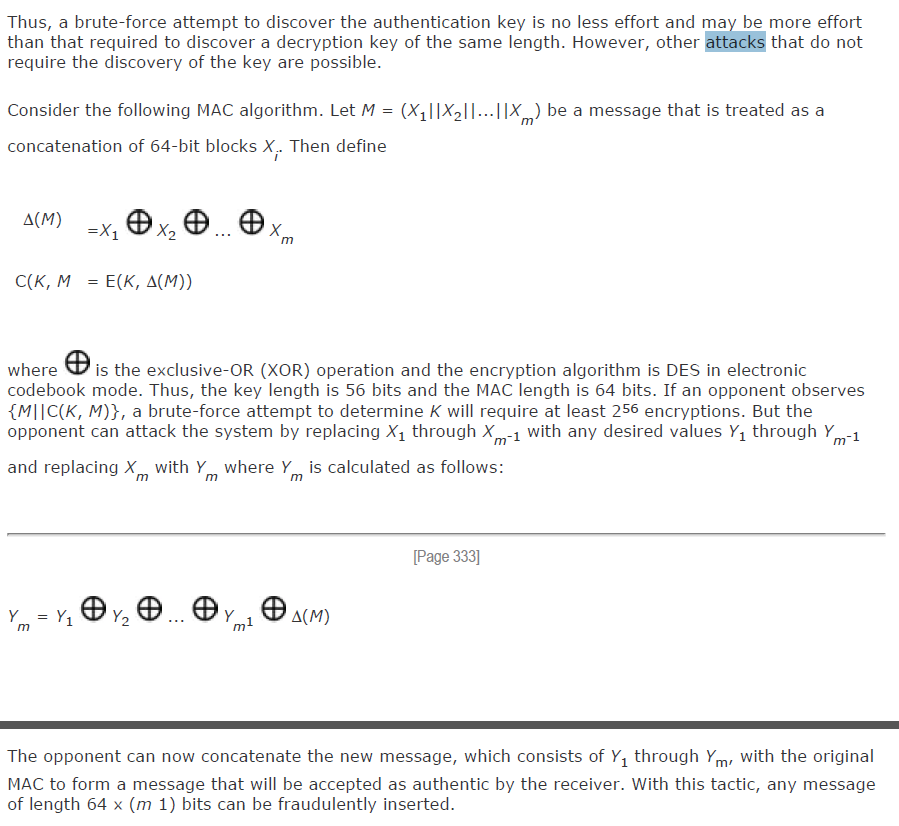
\includegraphics[width=1\textwidth]{img/128.png}
\end{figure}
\paragraph{2}
利用CBC-MAC(即FIPS PUB 313定义的数据认证算法)来生成消息认证码,安全吗?为什么?

\begin{figure}[htbp]
	\centering
	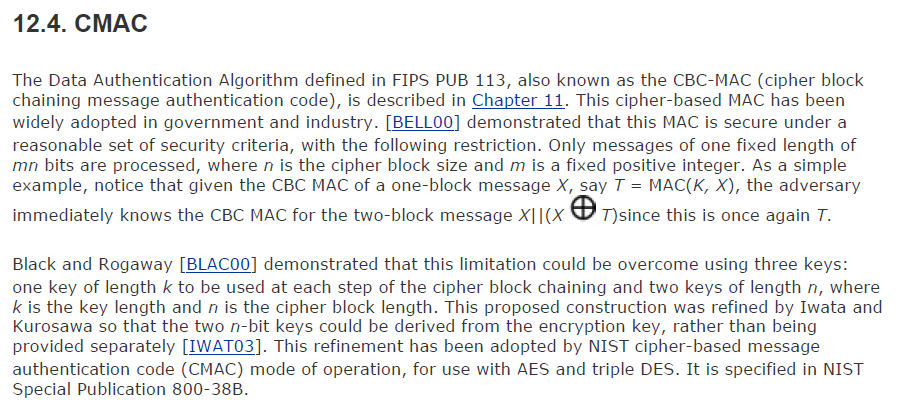
\includegraphics[width=1\textwidth]{img/124.png}
\end{figure}
\section{第13章 数字签名}
\paragraph{13.1}
List two disputes that can arise in the context of message authentication.

Suppose that John sends an authenticated message to Mary. The following disputes that could arise: 1. Mary may forge a different message and claim that it came from John. Mary would simply have to create a message and append an authentication code using the key that John and Mary share. 2. John can deny sending the message. Because it is possible for Mary to forge a message, there is no way to prove that John did in fact send the message.
\paragraph{13.2}
What are the properties a digital signature should have?

\begin{enumerate}[(a)]
    \item It must be able to verify the author and the date and time of the signature. 
    \item It must be able to authenticate the contents at the time of the signature.
    \item The signature must be verifiable by third parties, to resolve disputes.
\end{enumerate}
\paragraph{13.5}
In what order should the signature function and the confidentiality function be applied to a message, and why?

It is important to perform the signature function first and then an outer confidentiality function. In case of dispute, some third party must view the message and its signature. If the signature is calculated on an encrypted message, then the third party also needs access to the decryption key to read the original message. However, if the signature is the inner operation, then the recipient can store the plaintext message and its signature for later use in dispute resolution.
\paragraph{13.6}
What are some threats associated with a direct digital signature scheme?

1. The validity of the scheme depends on the security of the sender's private key. If a sender later wishes to deny sending a particular message, the sender can claim that the private key was lost or stolen and that someone else forged his or her signature. 2. Another threat is that some private key might actually be stolen from X at time T. The opponent can then send a message signed with X's signature and stamped with a time before or equal to T
\section{第14章 密钥管理和分发}
\paragraph{14.1}
Explain why man-in-the-middle attacks are ineffective on the secret key distribution protocol discussed in Figure 14.3.
\begin{figure}[htbp]
	\centering
	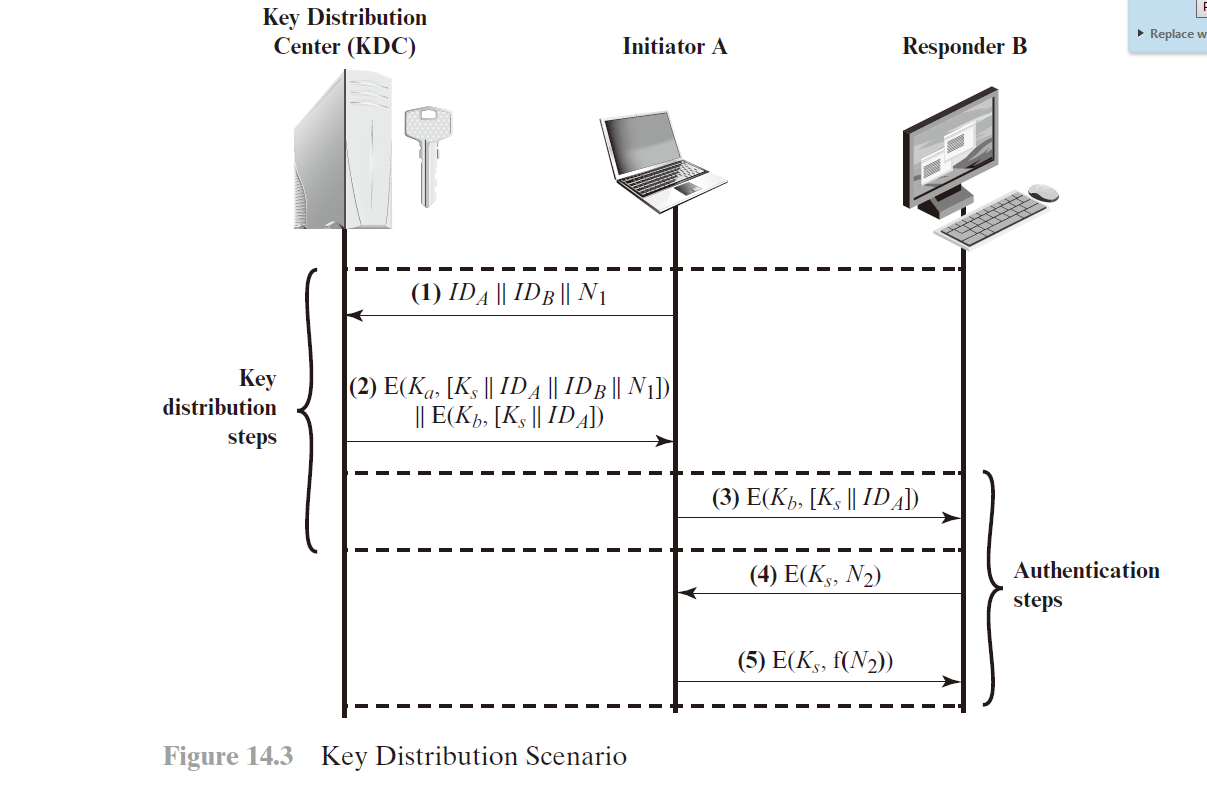
\includegraphics[width=1\textwidth]{img/141.png}
\end{figure}
中间人没有Ka,也就没法解密出服务器发给他的(2),他不能取(3)出发给B,B也就不相信他。
\paragraph{14.2}
What is the major issue in end to end key distribution? How does the key hierarchy concept address that issue?

\begin{figure}[htbp]
	\centering
	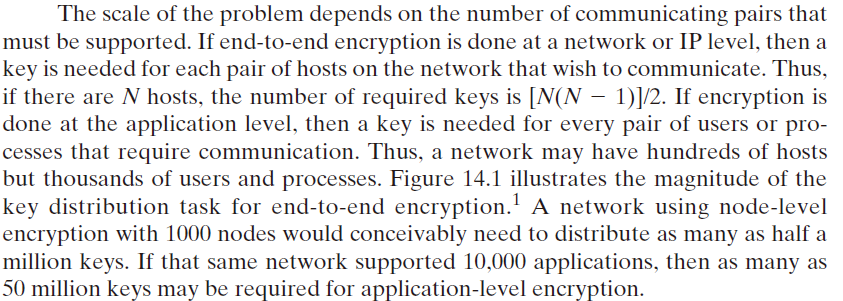
\includegraphics[width=1\textwidth]{img/142.png}
\end{figure}
主要的问题是,key的数量非常庞大。对于N个节点的网络,需要N*(N-1)/2对key。这些key如何分发和管理成为了问题。

用key hierarchy配合 option 4的方法, 所有节点和一个中间节点c共享密钥,然后任意两个节点间a b的密钥,通过c来协商和分发。 这样,不通信的节点间就不需要密钥,需要通信时候可以通过c按需协商和分发密钥。
\paragraph{14.3}
What is a nonce?

A nonce is a value that is used only once, such as a timestamp, a counter, or a random number; the minimum requirement is that it differs with each transaction.
\paragraph{14.6}
List four general categories of schemes for the distribution of public keys.

Public announcement. Publicly available directory. Public-key authority. Public-key certificates
\paragraph{14.8}
What is a public-key certificate?

A public-key certificate contains a public key and other information, is created by a certificate authority, and is given to the participant with the matching private key. A participant conveys its key information to another by transmitting its certificate. Other participants can verify that the certificate was created by the authority.
\paragraph{14.9}
What are the requirements for the use of a public-key certificate scheme?

1. Any participant can read a certificate to determine the name and public key of the certificate's owner. 2. Any participant can verify that the certificate originated from the certificate authority and is not counterfeit. 3. Only the certificate authority can create and update certificates. 4. Any participant can verify the currency of the certificate.
\paragraph{14.10}
What is the purpose of the X.509 standard?

X.509 defines a framework for the provision of authentication services by the X.500 directory to its users. The directory may serve as a repository of public-key certificates. Each certificate contains the public key of a user and is signed with the private key of a trusted certification authority. In addition, X.509 defines alternative authentication protocols based on the use of public-key certificates.
\paragraph{14.11}
What is a chain of certificates?

A chain of certificates consists of a sequence of certificates created by different certification authorities (CAs) in which each successive certificate is a certificate by one CA that certifies the public key of the next CA in the chain.
\paragraph{14.12}
How is an X.509 certificate revoked?

The owner of a public-key can issue a certificate revocation list that revokes one or more certificates.
\paragraph{14.2}
会话密钥和主密钥有什么不同?

A session key is a temporary encryption key used between two principals. A master key is a long-lasting key that is used between a key distribution center and a principal for the purpose of encoding the transmission of session keys. Typically, the master keys are distributed by noncryptographic means.
\section{第15章 用户认证}
\paragraph{15.2}
List three general approaches to dealing with replay attacks.

1. Attach a sequence number to each message used in an authentication exchange. A new message is accepted only if its sequence number is in the proper order. 2. Party A accepts a message as fresh only if the message contains a timestamp that, in A's judgment, is close enough to A's knowledge of current time. This approach requires that clocks among the various participants be synchronized. 3. Party A, expecting a fresh message from B, first sends B a nonce (challenge) and requires that the subsequent message (response) received from B contain the correct nonce value.
\paragraph{15.4}
What problem was Kerberos designed to address?

The problem that Kerberos addresses is this: Assume an open distributed environment in which users at workstations wish to access services on servers distributed throughout the network. We would like for servers to be able to restrict access to authorized users and to be able to authenticate requests for service. In this environment, a workstation cannot be trusted to identify its users correctly to network services.
\begin{figure}[htbp]
	\centering
	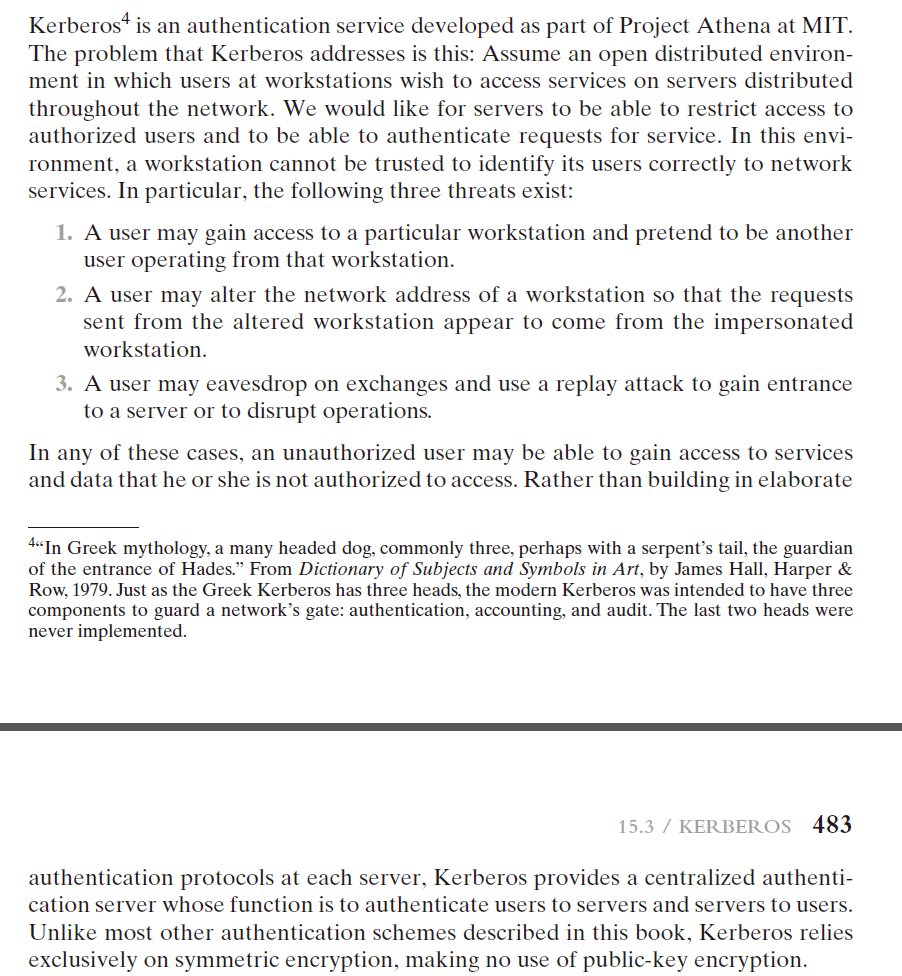
\includegraphics[width=1\textwidth]{img/154.png}
\end{figure}
\paragraph{15.10}
In Kerberos, when Bob receives a Ticket from Alice, how does he know it is not genuine? 

如果Alice是假的,他就不能用KA解密出KDC发来的 ,也就不能有用Bob的KB加密的消息 。 对于一个假的消息,Bob解密后发现消息格式里的A B L这些信息不合法,就知道Alice是假的了。
\paragraph{15.11}
In Kerberos, how does Bob know that the received token is not corresponding to Alice’s?

在Kerberos,当Bob收到一个来自于Alice的票据,如何得知其是否真实?如何得知其确实来自于Alice?
是否真实见上一题。
如果消息来源不是Alice,那  里面的A就一定不是alice,而且这个消息没法伪造,因为只有KDC才知道KB.

\paragraph{15.12}
In Kerberos, how does Alice know that a reply to an earlier message is from Bob?

在Kerberos,当Alice收到一个回复,她如何得知该消息来自于Bob(且是Bob最新的回复)
 
Alice发给Bob的信息是用KS加密的,这个KS是只有Alice和Bob和KDC 才知道的。 只有BOB才能成功解密 ,并且发出挑战的应答 。
Alice知道N 和L,L里有时间戳信息。  Alice收到N+1后,减1也就得到了N, 然后查找N对应的L,即可知道时间戳信息。
也许这题是想问如果有多个Bob: bob1 bob2,怎么知道来自哪个bob?
如果bob1 bob2的ip不同,那就好办。
否则就尝试用bob1的ks 和bob2的ks解密,看哪个解密出来的跟某一个N匹配就可以了。
\end{document}